\documentclass{standalone}
\usepackage{tikz}
\usetikzlibrary{patterns, positioning}


\begin{document}
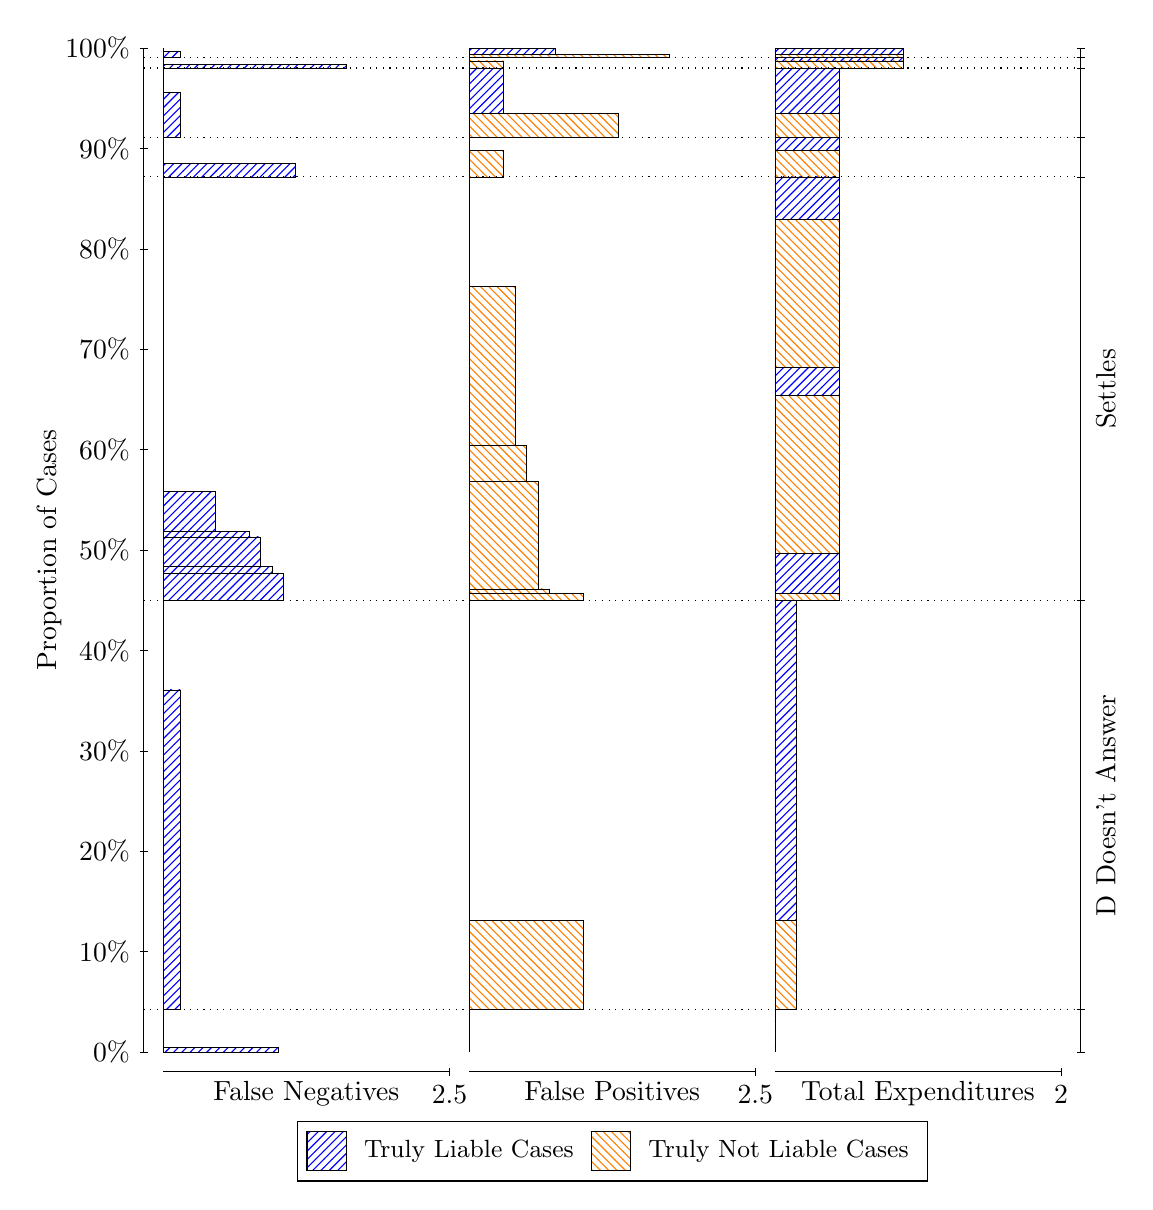
\begin{tikzpicture}
\draw[black, very thin] (1.5,1.75) -- (1.5,14.5);
\node[rotate=90, text=black, anchor=center] at (0.3, 8.125) {Proportion of Cases};
\draw[black, very thin] (1.45,1.75) -- (1.55,1.75);
\node[text=black, anchor=east] at (1.45, 1.75) {0\%};
\draw[black, very thin] (1.45,3.025) -- (1.55,3.025);
\node[text=black, anchor=east] at (1.45, 3.025) {10\%};
\draw[black, very thin] (1.45,4.3) -- (1.55,4.3);
\node[text=black, anchor=east] at (1.45, 4.3) {20\%};
\draw[black, very thin] (1.45,5.575) -- (1.55,5.575);
\node[text=black, anchor=east] at (1.45, 5.575) {30\%};
\draw[black, very thin] (1.45,6.85) -- (1.55,6.85);
\node[text=black, anchor=east] at (1.45, 6.85) {40\%};
\draw[black, very thin] (1.45,8.125) -- (1.55,8.125);
\node[text=black, anchor=east] at (1.45, 8.125) {50\%};
\draw[black, very thin] (1.45,9.4) -- (1.55,9.4);
\node[text=black, anchor=east] at (1.45, 9.4) {60\%};
\draw[black, very thin] (1.45,10.675) -- (1.55,10.675);
\node[text=black, anchor=east] at (1.45, 10.675) {70\%};
\draw[black, very thin] (1.45,11.95) -- (1.55,11.95);
\node[text=black, anchor=east] at (1.45, 11.95) {80\%};
\draw[black, very thin] (1.45,13.225) -- (1.55,13.225);
\node[text=black, anchor=east] at (1.45, 13.225) {90\%};
\draw[black, very thin] (1.45,14.5) -- (1.55,14.5);
\node[text=black, anchor=east] at (1.45, 14.5) {100\%};

\draw[black, very thin] (13.4,1.75) -- (13.4,14.5);
\draw[black, very thin] (13.35,1.75) -- (13.45,1.75);
\node[anchor=west] at (13.35, 1.75) {};
\draw[black, very thin] (13.35,2.2876) -- (13.45,2.2876);
\node[anchor=west] at (13.35, 2.2876) {};
\draw[black, very thin] (13.35,7.4802) -- (13.45,7.4802);
\node[anchor=west] at (13.35, 7.4802) {};
\draw[black, very thin] (13.35,12.863) -- (13.45,12.863);
\node[anchor=west] at (13.35, 12.863) {};
\draw[black, very thin] (13.35,13.365) -- (13.45,13.365);
\node[anchor=west] at (13.35, 13.365) {};
\draw[black, very thin] (13.35,14.247) -- (13.45,14.247);
\node[anchor=west] at (13.35, 14.247) {};
\draw[black, very thin] (13.35,14.379) -- (13.45,14.379);
\node[anchor=west] at (13.35, 14.379) {};
\draw[black, very thin] (13.35,14.5) -- (13.45,14.5);
\node[anchor=west] at (13.35, 14.5) {};

\draw[black, very thin, pattern color=blue, pattern=north east lines] (1.75,1.75) rectangle (3.2033,1.8066);
\draw[black, very thin, pattern color=orange, pattern=north west lines] (1.75,1.8066) rectangle (1.75,2.2876);
\draw[black, very thin, pattern color=blue, pattern=north east lines] (1.75,2.2876) rectangle (1.968,6.3485);
\draw[black, very thin, pattern color=orange, pattern=north west lines] (1.75,6.3485) rectangle (1.75,7.4802);
\draw[black, very thin, pattern color=blue, pattern=north east lines] (1.75,7.4802) rectangle (3.276,7.8278);
\draw[black, very thin, pattern color=blue, pattern=north east lines] (1.75,7.8278) rectangle (3.1307,7.9167);
\draw[black, very thin, pattern color=blue, pattern=north east lines] (1.75,7.9167) rectangle (2.9853,8.2921);
\draw[black, very thin, pattern color=blue, pattern=north east lines] (1.75,8.2921) rectangle (2.84,8.3644);
\draw[black, very thin, pattern color=blue, pattern=north east lines] (1.75,8.3644) rectangle (2.404,8.8741);
\draw[black, very thin, pattern color=orange, pattern=north west lines] (1.75,8.8741) rectangle (1.75,12.863);
\draw[black, very thin, pattern color=blue, pattern=north east lines] (1.75,12.863) rectangle (3.4213,13.032);
\draw[black, very thin, pattern color=orange, pattern=north west lines] (1.75,13.032) rectangle (1.75,13.365);
\draw[black, very thin, pattern color=blue, pattern=north east lines] (1.75,13.365) rectangle (1.968,13.939);
\draw[black, very thin, pattern color=orange, pattern=north west lines] (1.75,13.939) rectangle (1.75,14.247);
\draw[black, very thin, pattern color=blue, pattern=north east lines] (1.75,14.247) rectangle (4.0753,14.288);
\draw[black, very thin, pattern color=orange, pattern=north west lines] (1.75,14.288) rectangle (1.75,14.379);
\draw[black, very thin, pattern color=blue, pattern=north east lines] (1.75,14.379) rectangle (1.968,14.459);
\draw[black, very thin, pattern color=orange, pattern=north west lines] (1.75,14.459) rectangle (1.75,14.5);
\draw[black, very thin, pattern color=orange, pattern=north west lines] (5.6333,1.75) rectangle (5.6333,2.2311);
\draw[black, very thin, pattern color=blue, pattern=north east lines] (5.6333,2.2311) rectangle (5.6333,2.2876);
\draw[black, very thin, pattern color=orange, pattern=north west lines] (5.6333,2.2876) rectangle (7.0867,3.4194);
\draw[black, very thin, pattern color=blue, pattern=north east lines] (5.6333,3.4194) rectangle (5.6333,7.4802);
\draw[black, very thin, pattern color=orange, pattern=north west lines] (5.6333,7.4802) rectangle (7.0867,7.5716);
\draw[black, very thin, pattern color=orange, pattern=north west lines] (5.6333,7.5716) rectangle (6.6507,7.6298);
\draw[black, very thin, pattern color=orange, pattern=north west lines] (5.6333,7.6298) rectangle (6.5053,8.9962);
\draw[black, very thin, pattern color=orange, pattern=north west lines] (5.6333,8.9962) rectangle (6.36,9.4569);
\draw[black, very thin, pattern color=orange, pattern=north west lines] (5.6333,9.4569) rectangle (6.2147,11.469);
\draw[black, very thin, pattern color=blue, pattern=north east lines] (5.6333,11.469) rectangle (5.6333,12.863);
\draw[black, very thin, pattern color=orange, pattern=north west lines] (5.6333,12.863) rectangle (6.0693,13.196);
\draw[black, very thin, pattern color=blue, pattern=north east lines] (5.6333,13.196) rectangle (5.6333,13.365);
\draw[black, very thin, pattern color=orange, pattern=north west lines] (5.6333,13.365) rectangle (7.5227,13.673);
\draw[black, very thin, pattern color=blue, pattern=north east lines] (5.6333,13.673) rectangle (6.0693,14.247);
\draw[black, very thin, pattern color=orange, pattern=north west lines] (5.6333,14.247) rectangle (6.0693,14.338);
\draw[black, very thin, pattern color=blue, pattern=north east lines] (5.6333,14.338) rectangle (5.6333,14.379);
\draw[black, very thin, pattern color=orange, pattern=north west lines] (5.6333,14.379) rectangle (8.1767,14.42);
\draw[black, very thin, pattern color=blue, pattern=north east lines] (5.6333,14.42) rectangle (6.7233,14.5);
\draw[black, very thin, pattern color=orange, pattern=north west lines] (9.5167,1.75) rectangle (9.5167,2.2311);
\draw[black, very thin, pattern color=blue, pattern=north east lines] (9.5167,2.2311) rectangle (9.5167,2.2876);
\draw[black, very thin, pattern color=orange, pattern=north west lines] (9.5167,2.2876) rectangle (9.7892,3.4194);
\draw[black, very thin, pattern color=blue, pattern=north east lines] (9.5167,3.4194) rectangle (9.7892,7.4802);
\draw[black, very thin, pattern color=orange, pattern=north west lines] (9.5167,7.4802) rectangle (10.334,7.5716);
\draw[black, very thin, pattern color=blue, pattern=north east lines] (9.5167,7.5716) rectangle (10.334,8.0813);
\draw[black, very thin, pattern color=orange, pattern=north west lines] (9.5167,8.0813) rectangle (10.334,10.093);
\draw[black, very thin, pattern color=blue, pattern=north east lines] (9.5167,10.093) rectangle (10.334,10.441);
\draw[black, very thin, pattern color=orange, pattern=north west lines] (9.5167,10.441) rectangle (10.334,12.326);
\draw[black, very thin, pattern color=blue, pattern=north east lines] (9.5167,12.326) rectangle (10.334,12.863);
\draw[black, very thin, pattern color=orange, pattern=north west lines] (9.5167,12.863) rectangle (10.334,13.196);
\draw[black, very thin, pattern color=blue, pattern=north east lines] (9.5167,13.196) rectangle (10.334,13.365);
\draw[black, very thin, pattern color=orange, pattern=north west lines] (9.5167,13.365) rectangle (10.334,13.673);
\draw[black, very thin, pattern color=blue, pattern=north east lines] (9.5167,13.673) rectangle (10.334,14.247);
\draw[black, very thin, pattern color=orange, pattern=north west lines] (9.5167,14.247) rectangle (11.152,14.338);
\draw[black, very thin, pattern color=blue, pattern=north east lines] (9.5167,14.338) rectangle (11.152,14.379);
\draw[black, very thin, pattern color=orange, pattern=north west lines] (9.5167,14.379) rectangle (11.152,14.42);
\draw[black, very thin, pattern color=blue, pattern=north east lines] (9.5167,14.42) rectangle (11.152,14.5);
\draw[black, dotted] (1.5,2.2876) -- (13.4,2.2876);
\draw[black, dotted] (1.5,7.4802) -- (13.4,7.4802);
\draw[black, dotted] (1.5,12.863) -- (13.4,12.863);
\draw[black, dotted] (1.5,13.365) -- (13.4,13.365);
\draw[black, dotted] (1.5,14.247) -- (13.4,14.247);
\draw[black, dotted] (1.5,14.379) -- (13.4,14.379);
\draw[black, very thin] (1.75,1.5) -- (5.3833,1.5);
\node[text=black, anchor=north] at (3.5667, 1.5) {False Negatives};
\draw[black, very thin] (5.3833,1.45) -- (5.3833,1.55);
\node[text=black, anchor=north] at (5.3833, 1.45) {2.5};

\draw[black, very thin] (5.6333,1.5) -- (9.2667,1.5);
\node[text=black, anchor=north] at (7.45, 1.5) {False Positives};
\draw[black, very thin] (9.2667,1.45) -- (9.2667,1.55);
\node[text=black, anchor=north] at (9.2667, 1.45) {2.5};

\draw[black, very thin] (9.5167,1.5) -- (13.15,1.5);
\node[text=black, anchor=north] at (11.333, 1.5) {Total Expenditures};
\draw[black, very thin] (13.15,1.45) -- (13.15,1.55);
\node[text=black, anchor=north] at (13.15, 1.45) {2};


\node[text=black, centered, rotate=90] at (13.72, 4.8839) {D Doesn't Answer};
\node[text=black, centered, rotate=90] at (13.72, 10.171) {Settles};





\draw (7.449999999999999,1.5) node[draw=none] (baseCoordinate) {};
\begin{scope}[align=center]
        \matrix[scale=0.5, draw=black, below=0.5cm of baseCoordinate, nodes={draw}, column sep=0.1cm]{
            \node[rectangle, draw, minimum width=0.5cm, minimum height=0.5cm, pattern color=blue, pattern=north east lines] {}; &
            \node[draw=none, font=\small, text=black] (B) {Truly Liable Cases}; &
            \node[rectangle, draw, minimum width=0.5cm, minimum height=0.5cm, pattern color=orange, pattern=north west lines] {}; &
            \node[draw=none, font=\small, text=black] (B) {Truly Not Liable Cases}; \\
            };
\end{scope}

\end{tikzpicture}
\end{document}